

\section{Ejercicio 3} \label{ej3}
	\begin{flushleft}
		\textit{Se pretende duplicar la duración del fragmento musical para lo cual se propone interpolar el
archivo de audio. No está permitido usar las funciones de matlab/octave que implementan la
interpolación directamente. Grafique el espectrograma de la nueva secuencia y compárela con
la obtenida en el Ejercicio 2.}
	\end{flushleft}

	\subsection{Interpolación}
		El algoritmo de interpolación lineal se simplifica al contar con el álgebra matricial propio del \textit{Matlab}. La rutina se resume a continuación:
		\begin{lstlisting}
	doble_audio = linspace(0,1,length(audio)*2);
	doble_audio(1:2:end) = audio;
	doble_audio(2:2:end-1)=(audio(2:end)-audio(1:end-1))/2+audio(1:end-1);
		\end{lstlisting}

	\subsection{Comparación de espectogramas}

		\begin{figure}[h!]
			\centering
			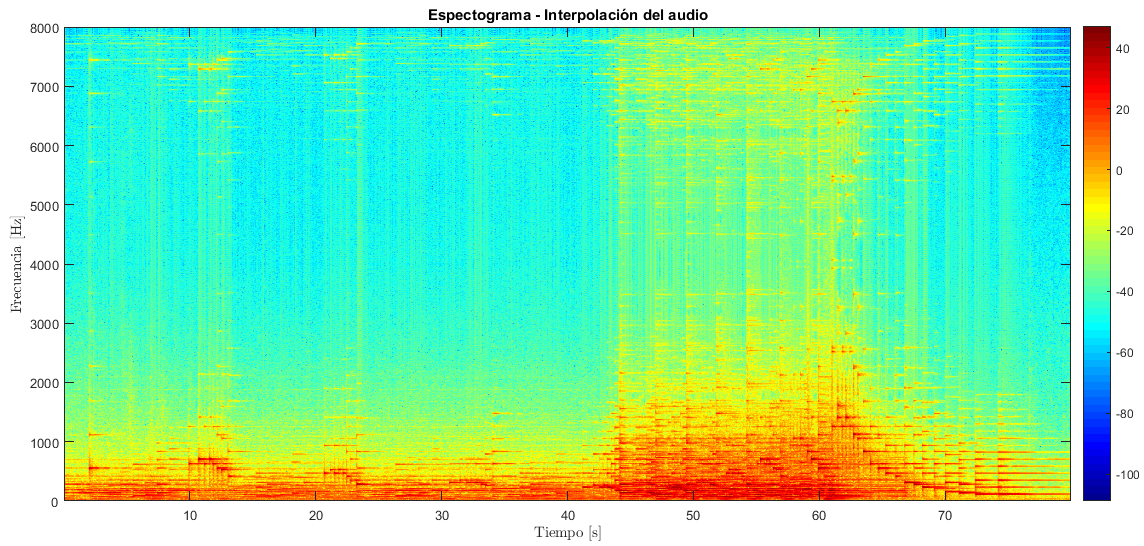
\includegraphics[scale=0.35]{3.png}
			\caption{Espectrograma de la señal interpolada.}
			\label{graf:ej3}
		\end{figure}
		Al interpolar la señal original, se obtiene el doble de muestras. Ante una misma $F_S$ (Figura \ref{graf:ej3}), la duración de la señal interpolada será el doble. A su vez, el espectro de frecuencias se comprime en 2.\\

		\graficarPNG{0.35}{3bis}{Espectrograma de la señal interpolada con $F_S^*=2 F_S$.}{graf:ej3bis}
		Realizando el espectograma de la señal interpolada con $F_S^*=2F_S$ (Figura \ref{graf:ej3bis}), se ve que las frecuencias son las mismas. Por lo tanto, si se reconstruyen ambas señales con sus respectivas frecuencias de muestreo se obtiene la misma señal.

		Por otro lado se ve que, debido a la interpolación, se presentan componentes de alta frecuencia que la original carecía ($f>\SI{8}{\kHz}$ con $F_S^*=2F_S$). Esto se debe a que, al ser periodica la DFT, la compresión del espectro copia parte del mismo espectro espejado. Por lo tanto, se propone realizar un filtrado pasabajos. El filtro a utilizar es una ventana rectangular en frecuencia. En la Figura \ref{graf:ej3bis_b} se expone el espectrograma de la señal interpolada y filtrada posteriormente.

		\graficarPNG{0.35}{3bbis}{Espectrograma de la señal interpolada filtrada con $F_S^*=2 F_S$.}{graf:ej3bis_b}

		Se podría interpretar que al aplicar el filtro la señal presentaría más ruido (zonas previamente en azul se grafican amarillas ahora). Esto se debe a que el graficador toma el valor más pequeño y lo define como azul oscuro. Se puede ver en las Figuras \ref{graf:ej3_comp} y \ref{graf:ej3_comp_b} que un mismo punto mantiene el valor de $z$ (denominada \textit{Index} en los gráficos). Por lo tanto, la señal filtrada es más fiel a la original dado que carece de los componentes de alta frecuencia parásitos.

		\graficarPNG{0.35}{3_comp}{Espectrograma para comparar - Interpolación sin filtro.}{graf:ej3_comp}
		\graficarPNG{0.35}{3b_comp}{Espectrograma para comparar - Interpolación con filtro.}{graf:ej3_comp_b}
